I had meetings the whole day! I caught a few minutes of the OptRL panel

\subsection{Panel at OptRL: Doina and Rich}

{\it Q: Are you happy with the balance of engineering vs. theory in RL?} \\

Doina: From my point of view we are trying to do good science and want to be building algorithms that we understand. What does it mean to understand algorithms? In the past this has often meant theory: convergence, PAC bounds, etc. But in some cases the theory can't yield understanding: vacuous bounds, hard to analyze cases, mismatch from real world, and so on. So, what we need is a concerted effort to make theory {\it meaningful}, and to make our experimental analysis more thorough in the sense of trying to understand what is going on, even in large scale experiments. Not necessarily theory but might point out new directions for theory. \\

Rich: Well, Doina, that's a very bold point of view you have that it's all about science! I have a hard time disagreeing. The engineering and experimental pieces are also really important. Every field has to deal with this clash. There shouldn't be a conflict. Any field, engineering or science, shoudl be like a conveyor belt: at one end you put in big ideas and practice, and at the other end you output a better deeper theoretical understanding. There is a natural drift toward experimental work. The goal is to increase understanding. You have to start with things you don't understand! We need new things on the conveyor belt so we understand more over time. \\

Doina: From a theoretical point of view, people say RL is very hard; but, that makes it very exciting! It's a good time to do theory in RL. After stalling for some number of years now we have momentum. \\

Rich: I totally agree. The field is hard because we're working with fundamental questions. I think about it as how intelligence works, how to achieve goals, and so on. The more we get to the core of these key problems, we should expect them to be challenging. Don't be discouraged when you do hard things! The real conclusion is that we have to value incremental progress on hard problems. A small amount of fundamental progress is a big deal. \\

\dnote{Had to run to meetings :(}



\subsection{Talk at Deep RL: Michael Littman on Assessing the Robustness of Deep RL Algorithms}

Background:
\begin{itemize}
    \item Started off interested in explainable RL: why does DQN choose the moves it does in Atari?
    
    \item Ended up wondering if any explanation at all is possible
    \item {\bf Punchline:} Generalizing Q values is hard!\cite{witty2018measuring}
\end{itemize}

Case study 1: Amidar! DQN can do extremely well on this game. \\

$\ra$ But: can we look at one of the moves and figure out {\it why} it made this decision? \\

To answer this:
\begin{itemize}
    \item An explanation is something that tells us how things would have been if something else happened.
    \item Tried causal interventions:
    \begin{enumerate}
        \item Idea one: Prefill one of the boxes! Think Pac-Man with some random pellets missing (couldn't have reached the state).
        
        $\ra$ Agent stops moving entirely and starts to be killed.
        
        \item Next up: get rid of the enemies! Same game (again think Pac man with no ghosts).
    \end{enumerate}
\end{itemize}

$\implies$ Takeaway here: DQN doesn't {\it really} know how to play the game! All it does is learn a good strategy, but it's very brittle. \\

Next up: investigate {\it saliency}. Ask: what makes big changes in action choice or value prediction if blurred out? What does the learned netwwork pay attention to? \\

$\ra$ Memorized movement! \\

So: maybe we're thinking about learning wrong. Let's go back to {\bf supervised learning}. How do we measure success?
\begin{itemize}
    \item how well it does on training set
    \item Interpolation: How well it does on test/validation set(s)
    \item Extrapolation: How well it does on out of distribution data
\end{itemize}

Analogues in RL, though:
\begin{itemize}
    \item Training examples $\ra$ On policy states
    \item Interpolation $\ra$ Off-policy states
    \item Exrapolation $\ra$ unreachable states.
\end{itemize}

Q: How can we test these different kinds of generalization/states in RL? \\

A: Different interventions! Off-policy: push to different states, force to unreachable states, and so on. \\

Evaluation Metrics: 1) Value Estimation Error (VEE): how far off is Q error?, and 2) Total Accumulated Reward (TAR). \\

\begin{figure}[h!]
    \centering
    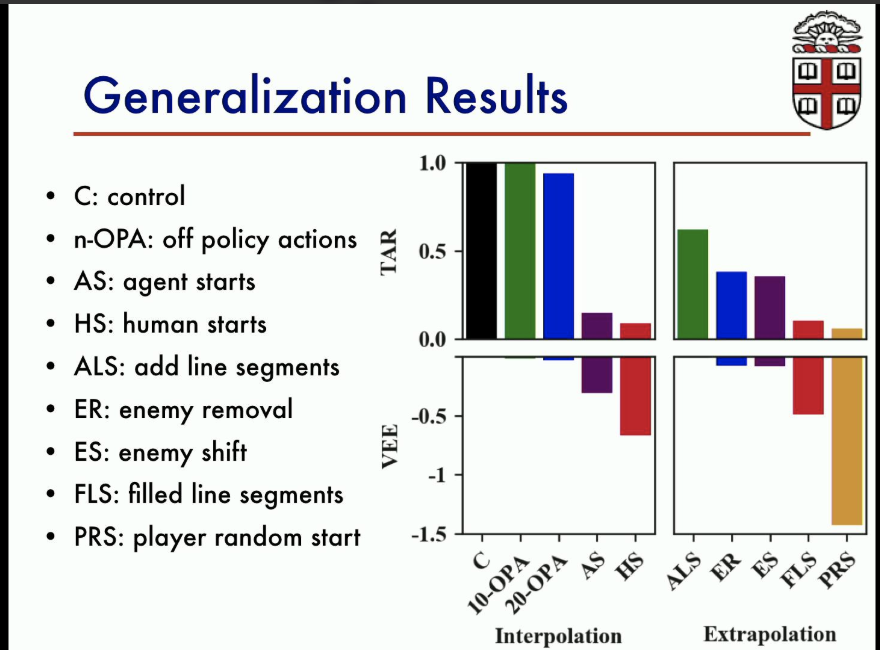
\includegraphics[width=0.7\textwidth]{figures/gen.png}
    \caption{Results on generalization types for RL}
    \label{fig:gen}
\end{figure}

Findings:
\begin{enumerate}
    \item Full results in Figure ~\ref{fig:gen}.
    \item VEE and TAR correlate.
    \item Novel states not recognized! Learned representation does not find the novel states to be similar to those seen in training (via activation analysis).
\end{enumerate}


Q: So how can we improve generalization? \\

A: Well, in supervised learning, we do a few things: 1) more data, and 2) less model (regularization). \\

Q: So how about in RL? \\

A: A few things: 1) can increase time, 2) Diversify training data, or 3) Regularize (reduce model capacity). \\

Tried these three changes to the learning procedure and inspected performance. \\

$\ra$ Finding: all three help! But not very much. \\

\begin{figure}[h!]
    \centering
    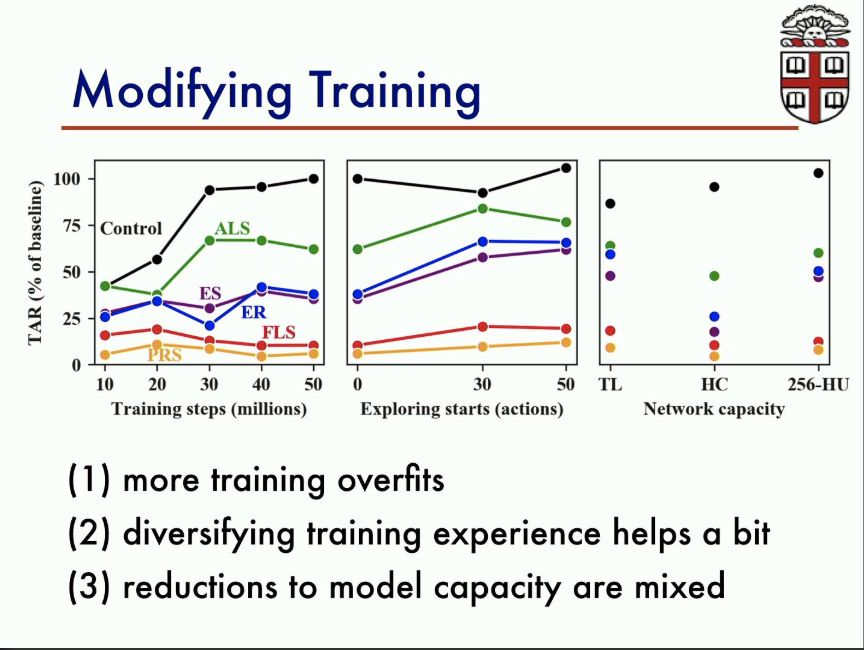
\includegraphics[width=0.7\textwidth]{figures/mod_train.png}
    \caption{Results for changing three aspects of training procedure}
    \label{fig:gen}
\end{figure}

Case Study: CoinRun \cite{cobbe2018quantifying}. New set of environments that are designed explicitly for studying generalization in RL.
\begin{itemize}
    \item Goal is to collect coin at the end of the level
    \item Agent spawns on the left
    \item Contains obstacles, enemies, level ends by death.
    \item Levels divided into three levels of difficulty.
    
    $\ra$ Results from \citet{cobbe2018quantifying} show {\it overfitting} curves, which is exciting to see in RL. See Figure \ref{fig:coinrun}.
\end{itemize}


\begin{figure}[h!]
    \centering
    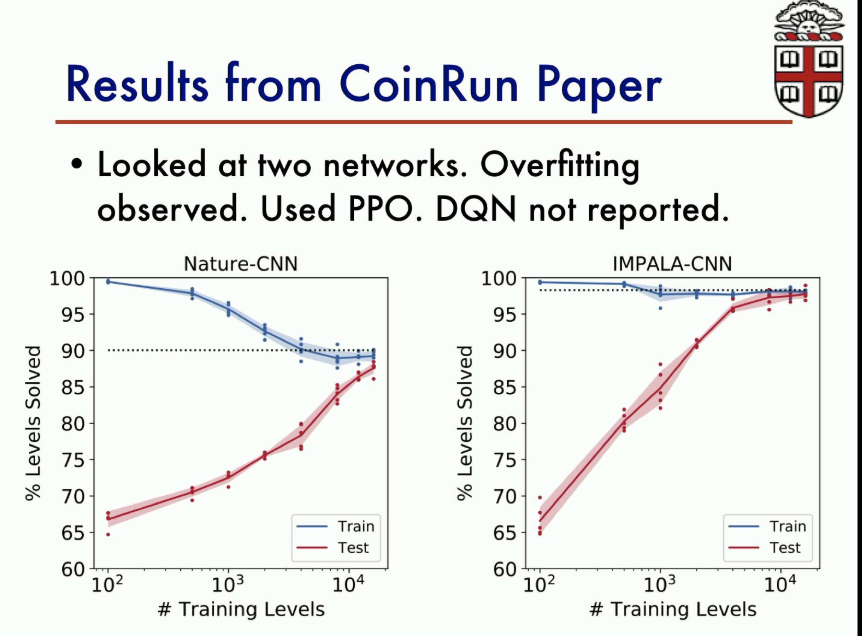
\includegraphics[width=0.7\textwidth]{figures/coin_run.png}
    \caption{Results on CoinRun domain from \citet{cobbe2018quantifying}}
    \label{fig:coinrun}
\end{figure}


But, the results on CoinRun were using a policy optimization method rather than DQN. \\

$\ra$ Tried to replicate with DQN, found the opposite result: it didn't work! Contacted the authors and they had found the same thing. \\

$\ra$ Later finding: DQN (and PPO) will generalize well with a lot of levels used (when the hard levels are removed). \\

Also studied prediction errors;
\begin{itemize}
    \item High prediction error associated with failure.
    \item Prediction error lower in training than testing.
    \item Training performance = testing performance  given enough data
\end{itemize}

Summary:
\begin{itemize}
    \item Good RL performance is seductive, but we need to look closer
    
    \item Analogy between RL and supervised learning is subtle
    \item DQN does not generalize well in Amidar, CoinRun, and some weak generalization in CoinRun difficulty 2.
    \item Found prediction error and internal representation 
    distance good predictors of poor generalization
    
    \item Adjusting training volume, model capacity, and exploration help, but only a bit.
\end{itemize}

\spacerule